\documentclass[11pt, a4paper]{article}
\usepackage[a4paper, margin = 0.7in]{geometry}
\usepackage{graphicx}
\usepackage{amsmath}
\usepackage{listings}
\usepackage{url}

\title{EE2703 Assignment 4 : Fourier Approximations}
\author{Aman Kumar EE19B066}
\date{March 10, 2021}

\begin{document}

\maketitle
\section{The assignment}
In this assignment we do the following-
\begin{itemize}
    \item We will fit two functions \textbf{exp(x)} and \textbf{cos (cos(x))} in the interval [0,2$\pi$) using the fourier series.
    \item Find fourier coefficients using integration.
    \item Find fourier coefficients using the method of least sqaures
    \item Compare the two results.
\end{itemize}
    \subsection{Introduction}
    The Fourier Series of a function $f(x)$ with period 2$\pi$ is computed as follows:
    \begin{equation*}
        f(x) = a_{0} + \sum_{n=1}^{\infty} \{a_{n}cos(nx) + b_{n}sin(nx)\}
    \end{equation*}
    Where, $a_n$ and $b_n$ are given by:
    \begin{equation*}
        a_{0} = \frac{1}{2\pi}\int_{0}^{2\pi} f(x)dx
    \end{equation*}
    \begin{equation*}
        a_{n} = \frac{1}{\pi}\int_{0}^{2\pi} f(x)cos(nx)dx
    \end{equation*}
    \begin{equation*}
        b_{n} = \frac{1}{\pi}\int_{0}^{2\pi} f(x)sin(nx)dx
    \end{equation*}
    \subsection{Things to do}
    Mainly the following things are asked in this assignment:
    \begin{itemize}
        \item Plot the functions over the interval [-2$\pi$,4$\pi$) and the expected functions generated by fourier series.
        \item Obtain the first 51 coefficients for the two functions above.
        \item Make different plots using “semilogy” and “loglog” and plot the
magnitude of the coefficients vs $n$. We have to plot this matrix:
            \[
            \begin{bmatrix}
                a_0\\
                a_1\\
                b_1\\
                ...\\
                a_{25}\\
                b_{25}
            \end{bmatrix}
            \]
        \item Find the same coefficients using the "Least squares approach".
        \item Compare the answers got by least squares and by the direct integration.
        \item Plot the function corresponding to fourier coefficients by least squares approach.
    \end{itemize}

\section{Assignment questions}
    \subsection{The given functions}
    The functions \textbf{exp(x)} and \textbf{cos(cos(x))} are defined using \textit{numpy.exp(x)} and \textit{numpy.cos()} respectively so that they can take vectors and input and return vectors as output. They are defined as:
    \begin{verbatim}
        def f1(x):
            return(np.exp(x))
        def f2(x):
            return(np.cos(np.cos(x)))
    \end{verbatim}

    The plot of the given functions, their expected fourier approximation plot and their plot by approximation by the method of least squares are given in Figure 1 and Figure 2. Since $exp(x)$ is not a periodic function, by fourier method we will get a periodic function with period 2$\pi$. It's graph over [0,2$\pi$) will be repeated as shown in Figure 1. But for $cos(cos(x))$, no such problem exists as it is a periodic function.
    \subsection{Obtaining Fourier coefficients through Integration}
    We are asked to compute the first 51 coefficients of the fourier series.
    To compute $a_n$ and $b_n$ we need to define two more functions $u(x,k,f) = f(x)cos(kx)$ and $v(x,k,f) = f(x)sin(kx)$. These function has a function as one of the arguments, this function is multiplied by $cos(nx)$ or $sin(nx)$ as required. They are defined as:
    \begin{verbatim}
        def u(x,f,k):
            return(f(x)*cos(k*x))
        def v(x,f,k):
            return(f(x)*sin(k*x))
    \end{verbatim}
    To perform integration \textbf{quad()} method is used of the module \textbf{scipy.integrate}. Since \textit{u(x,f,k)} and \textit{v(x,f,k)} both require 3 arguments, remaining two arguments i.e. f and k are passed by doing \textit{args = (f,k)}. The function to find coefficients is defined as:
    \begin{verbatim}
        def cal_coeff(f,coeffs):
            coeffs[0] += (1/(2*Pi))*quad(f,0,2*Pi)[0]
    
            for i in range(1,26):
                coeffs[2*i - 1] += (quad(u,0,2*Pi,args=(f,i))[0])/Pi
                coeffs[2*i] += (quad(v,0,2*Pi,args=(f,i))[0])/Pi
    \end{verbatim}
    \textbf{semilogy} plots of magnitude of coefficients are plotted in Figure 3 and Figure 5, and \textbf{loglog} are plotted in Figure 4 and Figure 6 for \textbf{exp(x)} and \textbf{cos(cos(x))} in that order with red circles.
    \subsection{Obtaining Fourier coefficients through Least squares approach}
    We define a vector $x$(called as \textbf{x\_}) going from 0 to 2$\pi$ in 400 steps and evaluate the function $f(x)$ at those $x$ values and call it b. Now we get the coefficients from the following matrix problem by \textbf{Least squares} approach.
    \[
    \begin{bmatrix}
        1 & cosx_1 & sinx_1 & ... & cos25x_1 & sin25x_1 \\
        1 & cosx_2 & sinx_1 & ... & cos25x_2 & sin25x_2 \\
        ... & ... & ... & ... & ... & ... \\
        1 & cosx_{400} & sinx_{400} & ... & cos25x_{400} & sin25x_{400}
    \end{bmatrix}
    \begin{bmatrix}
        a_0\\
        a_1\\
        b_1\\
        ...\\
        a_{25}\\
        b_{25}
    \end{bmatrix}
    =
    \begin{bmatrix}
        f(x_1)\\
        f(x_2)\\
        ...\\
        f(x_{400})
    \end{bmatrix}
    \]
    We call the matrix on the left \textbf{A}. Then the coefficient matrix \textbf{c} is given by:
    \begin{verbatim}
        c=lstsq(A,b)[0]
    \end{verbatim}
    
    The matrix \textbf{A} is calculated as follows:
    \begin{verbatim}
        A = np.zeros((400,51))
        A[:,0] = 1
        for i in range(1,26):
            A[:,2*i - 1] = np.cos(i*x_)
            A[:,2*i] = np.sin(i*x_)
    \end{verbatim}
    
    In my code the coefficients through this approach is found as follows:
    \begin{verbatim}
        def cal_coeff_lsq(A,f):
            if f == f1:
                b = f1(x_)
            elif f == f2:
                b = f2(x_)
            return(pl.lstsq(A,b,rcond=None)[0])
    \end{verbatim}
    \textbf{semilogy} plots of magnitude of coefficients obtained through this approach are plotted in Figure 3 and Figure 5, and \textbf{loglog} plot are plotted in Figure 4 and Figure 6 for \textbf{exp(x)} and \textbf{cos(cos(x))} in that order with green circles.
    \subsection{Comparing the two answers}
    We compare the answers got by least squares and by the direct integration by finding the absolute difference between the two sets of coefficients and finding the largest deviation. I did this by:
    \begin{verbatim}
    def Compare():
        return(max(abs(coeffs_f1 - coeffs_f1_ls)),max(abs(coeffs_f2 - coeffs_f2_ls)))
    \end{verbatim}
    Max deviation in the coefficients of $exp(x)$ : 1.3327308703352259\\
    Max deviation in the coefficients of $cos(cos(x))$ : 2.5428380512387945e-15
    \\\\
    Clearly, Our Predictions for $exp(x)$ are very poor compared to that of $cos(cos(x))$. This can be fixed by sampling at a larger number of points.  But this will be a small change in accuracy at a very large computational cost. Hence it isn't worth it as far as this assignment is concerned.
\section{Plots and Results}
    \subsection{The functions}
    We plot the functions $exp(x)$ and $cos(cos(x))$ in Figure 1 and Figure 2 respectively, along with the expected fourier apprixamation and approximation through least squares.
    \begin{figure}[!h]
        \centering
        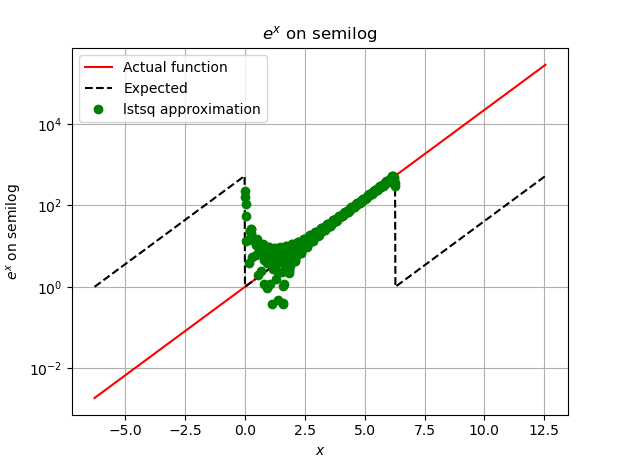
\includegraphics[scale = 0.7]{Figure 1.png}
        \caption{$exp(x)$}
        \label{fig:Figure 1}
    \end{figure}
    
    Here, we can see that there are large deviations in the approximation by least squares, this because $exp(x)$ is not a periodic function and to determine it's fourier series we periodically extended the function, thus creating discontinuities at intervals of 2$\pi$. Therefore at the first discontinuity of these intervals we see large deviations. We can also reduce the deviation by sampling at a very large number of points(as mentioned earlier).
    \begin{figure}[!h]
        \centering
        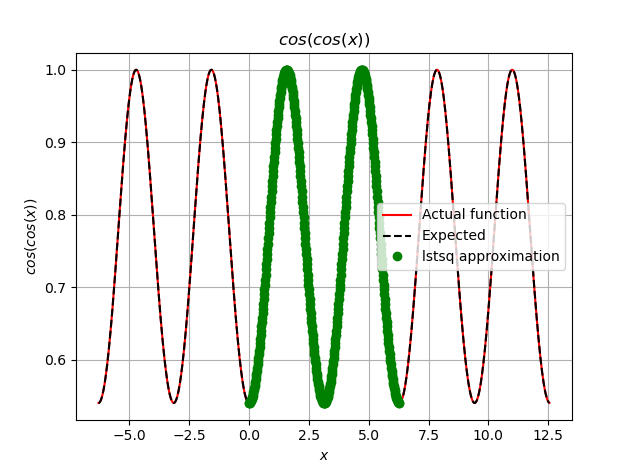
\includegraphics[scale = 0.8]{Figure 2.png}
        \caption{$cos(cos(x))$}
        \label{fig:Figure 2}
    \end{figure}
    
    However, there is almost no deviation from expected plot in the case of $cos(cos(x))$ as it is a periodic and continuous function. Hence, fourier series converges everywhere to the function.
    Code snippet used to plot the above two plots:
    \begin{verbatim}
def Plot_fn(f):
    y1 = f(x)
    y3 = f(x_)
    y3 = np.concatenate((y3,y3,y3))
    if f == f1:                       #If function is exp(x)
        Title = "$e^x$ on semilog"
        y2 = np.dot(A,coeffs_f1_ls)                                              
        pl.semilogy(x,y1,label="Actual function",color='red')                    
        pl.semilogy(x,y3.transpose(),label="Expected",color='black',linestyle='dashed')
        pl.semilogy(x_,y2,'go',label="lstsq approximation")                      
    elif f == f2:                    #If function is cos(cos(x))
        Title = "$cos(cos(x))$"
        y2 = np.dot(A,coeffs_f2_ls)                                              
        pl.plot(x,y1,label="Actual function",color='red')                        
        pl.plot(x,y3.transpose(),label="Expected",color='black',linestyle='dashed')
        pl.plot(x_,y2,'go',label="lstsq approximation")      
    \end{verbatim}
    \subsection{Coefficients}
    We plot the magnitude of coefficients for both the functions on \textbf{semilogy} and \textbf{loglog}. The coefficients obtained through both methods are plotted in the same plot. Code snippet used to plot the \textbf{semilog} and \textbf{loglog} plots(I've omitted non-important stuff):
    \begin{verbatim}
pl.semilogy(n,abs(coeffs_f1),'ro',label="$Integration$",linestyle='dashed',linewidth=1)
pl.semilogy(n,abs(coeffs_f1_ls),'go',label="$Least sqaures$",linestyle='dashed',linewidth=1)

pl.loglog(n,abs(coeffs_f1),'ro',label="$Integration$",linestyle='dashed',linewidth=1)
pl.loglog(n,abs(coeffs_f1_ls),'go',label="$Least sqaures$",linestyle='dashed',linewidth=1)

    
    \end{verbatim}
    \begin{figure}[!h]
        \centering
        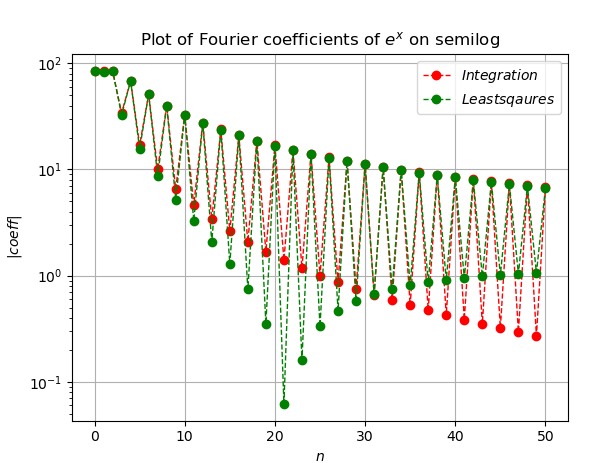
\includegraphics[scale = 0.8]{Figure 3.png}
        \caption{Coefficients of $exp(x)$ on semilogy}
        \label{fig:Figure 3}
    \end{figure}

    We can see here that this plot(semilogy) is not linear, while the plot in loglog is linear. Also we can see that value of coefficients($b_n$) found by the two methods are differing in some range.
    \begin{figure}[!h]
        \centering
        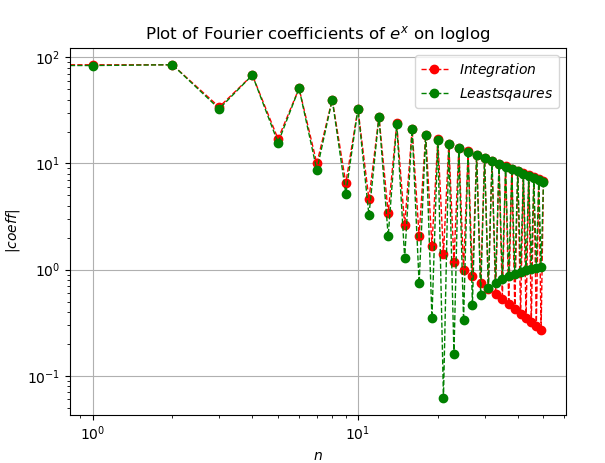
\includegraphics[scale = 0.8]{Figure 4.png}
        \caption{Coefficients of $exp(x)$ on loglog}
        \label{fig:Figure 4}
    \end{figure}
    
    We observe that the coefficients for $exp(x)$ do not decay as quickly as the coefficients for $cos(cos(x))$, which means $exp(x)$ has a lot(and higher) of frequencies in it's spectrum, while $cos(cos(x))$ is made up of very less number of frequencies.
    \begin{figure}[!h]
        \centering
        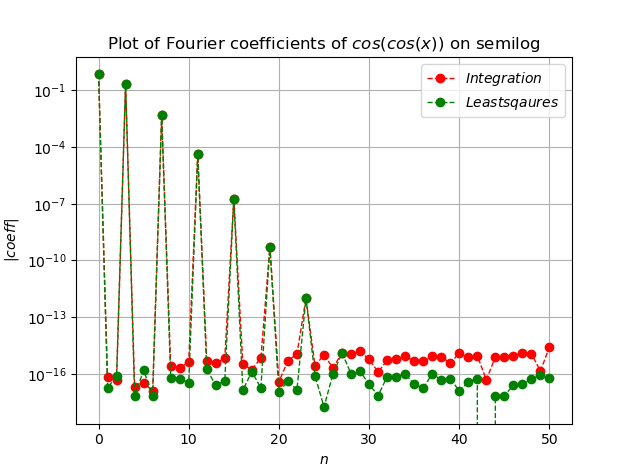
\includegraphics[scale = 0.8]{Figure 5.png}
        \caption{Coefficients of $cos(cos(x))$ on semilogy}
        \label{fig:Figure 5}
    \end{figure}
    
    Also, since $cos(cos(x))$ is an \textbf{even function} therefore its fourier sine series is zero. This is reflected in the plots as the coefficients $b_n$ are nearly zero($<10^{-15}$) while this is not the case for $exp(x)$ as it is not an even function.
    \begin{figure}[!h]
        \centering
        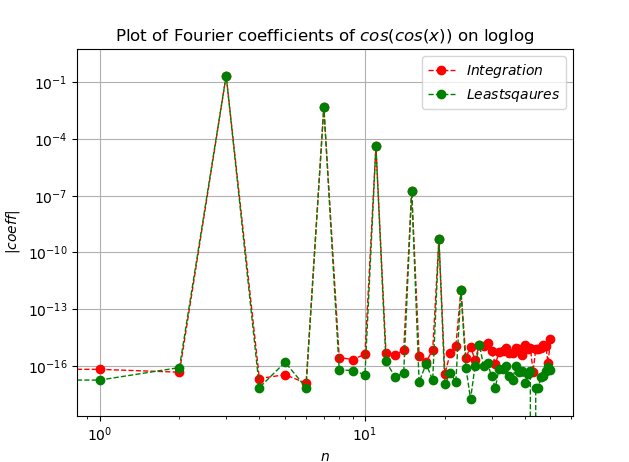
\includegraphics[scale = 0.7]{Figure 6.png}
        \caption{Coefficients of $cos(cos(x))$ on loglog}
        \label{fig:Figure 6}
    \end{figure}
    
    The coefficients for $cos(cos(x))$ are linear in semilogy whille non-linear in loglog. For $exp(x)$ $a_n$ and $b_n$ decay as $1/n^2$ and $1/n$, so $log(a_n)$ and $log(b_n)$ will be approximately proportional to $log(n)$. Thus loglog is linear. While in $cos(cos(x))$ the coefficients decay exponentially w.r.t n, hence semilog plot looks linear. 
\section{Concluions}
We have examined the case of approximating functions using their Fourier coefficients upto a threshold. We perform the same for two cases, one a continuous function, and the other a function with finite discontinuities. In the latter case, we found that the error in apprximation is more than that of continuous case.

The methods adopted in finding the Fourier coefficients have been evaluation through Euler's formulae(integration), as well an Least Square best fit approach. We notice close matching of the two methods in case of $cos(cos(x))$ while, there is a larger discrepancy in $exp(x)$.
\end{document}